\documentclass[12pt]{article}

\usepackage[margin=0.8 in]{geometry}
\usepackage{amsmath}
\usepackage{amssymb}
\usepackage{mathtools}
\usepackage{enumerate}
\usepackage{verbatim}
\usepackage{amsthm}
\usepackage{hyperref}
\usepackage{lipsum}

\title{}
%\content{}



\let \proj \undefined
\newcommand{\p}{\partial}
\newcommand{\R}{ \mathbb{R}}
\DeclareMathOperator{\proj}{proj}
\newcommand{\sS}{\mathscr{S}}
\DeclareMathOperator{\comp}{comp}
\newcommand{\A}{\mathcal{A}}
\newcommand{\D}{\mathcal{D}}
\newcommand{\e}{\epsilon}
\newcommand{\et}{\tilde{\e}}
\newcommand{\vr}{\vec{r}{}}
\newcommand{\vF}{\vec{F}}
\newcommand{\triple}{\iiint_E f(x,y,z)dV}
\renewcommand{\lg}{\langle}
\newcommand{\rg}{\rangle}
\newcommand{\Q}{\frac{\p Q}{\p x}}
\renewcommand{\P}{\frac{\p P}{\p y}}
\newcommand{\vi}{\vec{i}}
\newcommand{\vj}{\vec{j}}
\newcommand{\vk}{\vec{k}}
\DeclareMathOperator{\curl}{curl}
\newcommand{\n}{\nabla}
\newcommand{\px}{\frac{\p }{\p x}}
\newcommand{\py}{\frac{\p }{\p y}}
\newcommand{\pz}{\frac{\p }{\p z}}
\DeclareMathOperator{\rot}{rot}
\let \div \undefined
\DeclareMathOperator{\div}{div}



\let\implies\Rightarrow

\newenvironment{sol}
  {\begin{proof}[Solution]}
  {\end{proof}
  
  }
\newtheorem{exm}{Example}
\newtheorem{exr}{Exercise}
\newtheorem{thm}{Theorem}
\newtheorem{defn}{Definition}


\begin{document}
\section*{Curl, Divergence and Laplacian}
What to know:
\begin{enumerate}
\item The definition of curl and it two properties, that is, theorem 1, and be able to tell a vector field of clearly nonzero $\curl$ from one with clearly zero $\curl$.
\item The definition of divergence and it two properties, that is, if $\div \vF\neq 0$ then  $\vF$ can't be written as the $\curl$ of another field, and be able to tell a vector field of clearly nonzero,positive or negative divergence from the picture.
\item Know the definition of the Laplace operator
\item Know what kind of objects those operator take as input and what they give as output.
\end{enumerate}



\subsection*{The $\curl$ operator}
Let's look at two plots of vector fields:

\begin{figure}[h]
\centering
\parbox{5cm}{
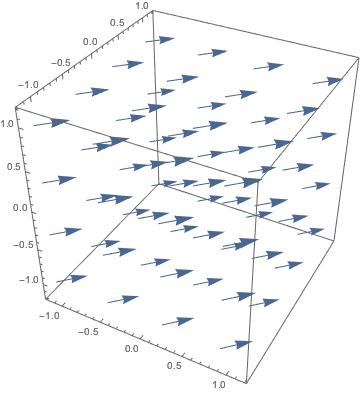
\includegraphics[width=5cm]{noncurly.jpeg}
\caption{The vector field $\lg -y,x,0\rg.$}
\label{fig1}}
\qquad
\begin{minipage}{5cm}
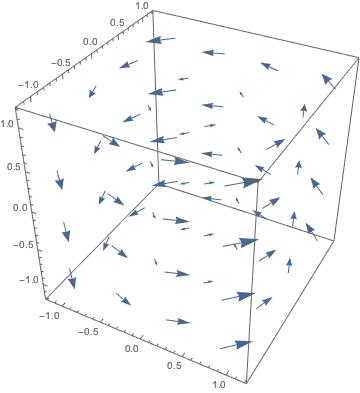
\includegraphics[width=5cm]{curly.jpeg}
\caption{The vector field $\lg 1,1,0\rg$}
\label{fig2}
\end{minipage}
\end{figure}

We can observe that the second one looks like it is rotating around the $z$ axis. We'd like to be able to predict this kind of behavior without having to look at a picture.  We also promised to find a criterion that checks whether a vector field is conservative in $\R^3$.

Both of those goals are accomplished using a tool called the \textbf{curl operator}, even though neither of those two properties is exactly obvious from the definition we'll give.

\begin{defn}
Let $\vF=\lg P,Q,R\rg $ be a vector field in $R^3$, where $P$, $Q$ and $R$ are continuously differentiable. We define the \textbf{curl operator}: \begin{equation}
\curl \vF=\left(\frac{\p R}{\p y}-\frac{\p Q}{\p z}\right)\vi +\left (\frac{\p P}{\p z}-\frac{\p R}{\p x}\right )\vj+\left( \frac{\p Q}{\p x}-\frac{\p P}{\p y}\right )\vk.
\end{equation} 
\end{defn}

\textbf{Remarks:}
\begin{enumerate}
\item The input of $\curl $ is a vector field in $\R^3$ and the resulting object $\curl\vF$ is a vector field in $\R^3$  itself. If you wanted to make some sense of $\curl $ for a vector field in 2 dimensions you could insert a third component equal to 0 in your vector field and use the above formula.
\item You can easily remember curl using the following informal determinant formula. We can formally write $\n=\lg \px,\py,\pz\rg$ and \begin{equation}
\curl \vF=\begin{tabular}{|c c c|}
$\vi$ & $\vj$ & $\vk$ \\ 
$\px$ & $\py$ & $\pz$ \\
$P$ & $Q$ & $R$ \\ 
\end{tabular} =\n\times\vF.\label{eqn1}
\end{equation}
\item Other popular notations in literature are $\n\times\vF$ and $\rot \vF$.
\end{enumerate}

\subsubsection*{Properties}
\begin{enumerate}
\item Conservative Vector fields.

Let's start with an exercise:
\begin{exr}
Let $\vF=\n f$ be a conservative vector field in $\R^3$. Compute $\curl \vF$.
\end{exr}


If you did the previous exercise, you'd see that $\curl \n f=0$ identically! In fact, we have the following:
\begin{thm} If $\vF$ is a continuously differentiable vector field \textbf{defined on all of $\R^3$} then $\vF$ is conservative \textbf{if and only if} $$\curl\vF=0$$ \textbf{everywhere on $\R^3$}.
\end{thm}

A (very informal) way to remember this, if you've taken a class on linear algebra: In linear algebra, the determinant of a matrix is zero if one line is a multiple of another. If $\vF$ is conservative, the third line in the determinant in \eqref{eqn1} becomes $\lg \frac{\p f}{\p x},\frac{\p f}{\p y},\frac{\p f}{\p z}\rg$, which can be very informally be thought of as a ``multiple'' of $\n=\lg \px,\py,\pz\rg$, which is the second row, by $f$. The behavior in those cases is similar, but the reason why it happens is slightly different: In the matrix case it's the fact that multiplication of scalars is commutative (that is, $a\cdot b=b\cdot a$), whereas in the $\curl$ case it's the fact that the mixed second partial derivatives of $f$ are equal (Clairaut's Theorem).



\item \textbf{Rotations}

The $\curl$ operator encodes information about infinitesimal rotations of a vector field. Think of a small plastic ball inside the stream of a river. If the ball rotates around itself, this means that the curl is nonzero. The $\curl$ is then parallel to the axis of rotation, and its direction can be found using the right hand rule.

\end{enumerate}
\textbf{${}^*$ An optional comment:}

In physics textbooks (or wikipedia), you might see this (or a seemingly slightly more general) mysteriously looking definition of $\curl$, at t a point $p$:
\begin{equation}
\curl\vF(p)\cdot\vec{n}:=\lim_{\e\to 0}\frac{1}{A(D_\e)}\int_c \vF\cdot d\vr,
\end{equation}
where $D_\e$ is a small disk of radius $\e$ centered at $p$, lying on the plane through $p$ and normal to $\vec{n}$. Also, $c$ is the boundary of this disk, oriented according to the right hand rule with respect to $\vec{n}$. 

Trying to understand how this definition works, if we replace $\vec{n}$ with, say, $\lg 0,0,1\rg$, we find that the $z$ component of $\curl$ is the (normalized) work produced by the vector field along infinitesimal circular paths, which measures infinitesimal rotation about the $z$ axis. Similarly, you can do something like that for $\vec{n}=\lg 1,0,0\rg$ and $\vec{n}=\lg 0,1,0\rg$. This weird definition will make more sense once we get to Stokes' theorem.


\subsection*{The Divergence operator}
The next operator we'll talk about is called a divergence. Again, let's look at Figures \ref{fig3}, \ref{fig4} and \ref{fig5}.
\begin{figure}[h]
\minipage{0.32\textwidth}
  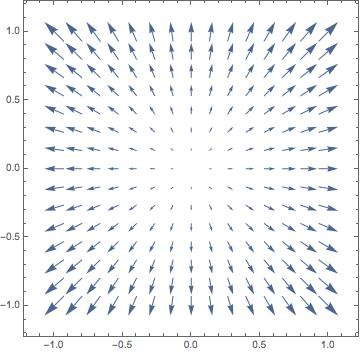
\includegraphics[width=\linewidth]{posdiv.jpeg}
  \caption{}\label{fig3}
\endminipage\hfill
\minipage{0.32\textwidth}
  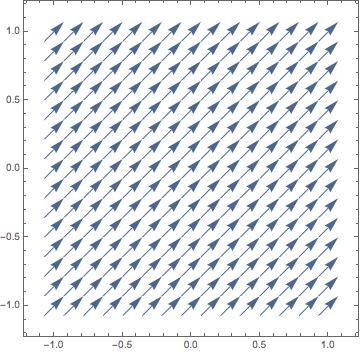
\includegraphics[width=\linewidth]{zerdiv.jpeg}
  \caption{}\label{fig4}
\endminipage\hfill
\minipage{0.32\textwidth}%
  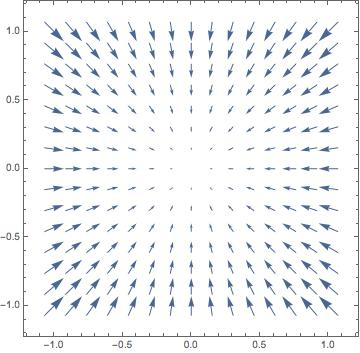
\includegraphics[width=\linewidth]{negdiv.jpeg}
  \caption{}\label{fig5}
\endminipage
\end{figure}

Suppose that the vector fields above represent the velocity vector fields of a fluid, and then imagine a drop of paint falling in each one of them? How would you expect its area to behave in each case? Again, we'd like a tool that would allow us to obtain this type of information without having to look at a picture. Our tool is called Divergence, and it works perfectly fine in any dimension.

We will defined as follows, in 2 dimansions:

\begin{defn}
The divergence operator of a \textbf{vector field} $\vF=\lg P,Q \rg$, where $P, Q$ are continuously differentiable, is defined as \begin{equation}
\div\vF=\frac{\p P}{\p x}+\frac{\p Q}{\p y}.
\end{equation}
\end{defn}

In three dimensions:

\begin{defn}
The divergence operator of a \textbf{vector field} $\vF=\lg P,Q,R \rg$, where $P, Q, R$ are continuously differentiable, is defined as \begin{equation}
\div\vF=\frac{\p P}{\p x}+\frac{\p Q}{\p y}+\frac{\p R}{\p z}.
\end{equation}
\end{defn}

\textbf{Remark:} Note that the divergence takes a vector field $\vF$ as input and $\div\vF$ is a scalar function.

\subsubsection*{Properties}

Why do we like divergence? For two reasons.
\begin{enumerate}
\item  It describes the extent to which a vector field behaves like a source/ sink. In Figures \ref{fig3}, \ref{fig4} and \ref{fig5} we can see vector fields with positive, zero and negative divergence, respectively. 
\item Do this exercise:
\begin{exr}
Let $\vF$ be a vector field in $\R^3$. Compute $\div\curl\vF$. 
\end{exr}
If you did the exercise, you should find 0. This tells us that if $\div \vec{G}\neq 0$ even at one point, then $\vec{G}$ can't be written as the $\curl $ of another vector field.
\end{enumerate}

\textbf{${}^*$ Another optional comment}


As with $\curl$, wikipedia gives a cumbersome definition of the divergence, which simplified and applied to two dimensions would be $$\div\vF(p)=\lim_{\e\to 0}\frac{1}{A(D_\e)}\int_{c_e} \vF\cdot \vec{n}ds,$$ where $c_\e$ is a positively oriented circle of radius $\e$ centered at $p$, $\vec{n}$ is the unit length outer pointing vector field to $c_\e$ and $A(D_\e)$ is the area of the disk of radius $\e$ centered at $p$. In a sense, you could say that the integral on the right hand side captures the ``amount'' of vector field exiting the disk cantered at $p$ with radius $\e$, so the divergence captures the corresponding infinitesimal quantity. It can be shown that the two definitions agree, feel free to ask if you are interested!




\subsubsection*{The Laplace Operator}
Perhaps the most commonly appearing operator in the study of Partial Differential Equations is the Laplace operator or Laplacian, defined as follows:
\begin{defn}
If $f(x,y,z)$ is a twice continuously differentiable scalar function, $$\Delta f=\div (\n f)=\frac{\p^2f}{\p x^2}+\frac{\p^2f}{\p y^2}+\frac{\p^2f}{\p z^2}.$$
\end{defn}
\textbf{Remark:} The Laplace operator takes a scalar function $f$ as input and $\Delta f$ is a scalar function.

It appears in the mathematical description of problems like propagation of sound waves or heat. The functions satisfying $\Delta f \equiv 0$ are called \textbf{harmonic}, and they have very strong and interesting properties. The study of harmonic functions is called \textbf{harmonic analysis}.







\end{document}

